\documentclass[a4paper, 11pt]{article}
\usepackage{comment} 
\usepackage{fullpage} 
\usepackage[spanish]{babel} 
\selectlanguage{spanish}
\usepackage[utf8]{inputenc}
\usepackage{float} 
\usepackage{graphicx}
\usepackage{ marvosym }
\usepackage{amsthm}
\usepackage{amsmath}
\usepackage[sort&compress, numbers]{natbib}
\usepackage{amssymb}
\usepackage{hyperref}
%\hypersetup{colorlinks=True, citecolor=blue}
\hypersetup{colorlinks=true, citecolor=green, urlcolor=blue}

\begin{document}
\begin{center}
\LARGE \bf Pr\'actica 9\\ Interacciones entre partículas
\end{center}

\vspace{1cm} 
\noindent\textbf {Edson Edgardo Samaniego Pantoja} \hfill \textbf{Materia:} Simulación computacional 
\hfill \\
\textbf{Fecha} \today  
\vspace{1cm} 

\section{Introducción}
En la práctica nueve se simula las interacciones entre partículas para fenómenos que ocurren a nivel electrón, tales fenómenos son de atracción y repulsión de cargas, de tal manera que cargas de un mismo signo producen una repulsión mientras cargas opuestas resultan en una atracción. 
\section{Metodología}
La simulación de partículas \texttt{n} y sus interacciones son dadas en código que se obtiene en el repositorio de Schaeffer \cite{elisa} y es explicado desde su pagina \cite{dra}. Cada partícula contiene una carga, la magnitud de la fuerza estará proporcional a la diferencia de magnitud de las cargas (mayores diferencias resultando en fuerzas mayores), y además la fuerza será inversamente proporcional a la distancia euclidiana entre las partículas.

\section{Objetivo}
Como objetivo de la práctica, se debe agregar a cada partícula una masa y hacer que la masa cause fuerzas gravitacionales (atracciones) además de las fuerzas causadas por las cargas. Así como estudiar la distribución de velocidades de las partículas y verificar gráficamente que esté presente una relación entre los tres factores: la velocidad, la magnitud de la carga, y la masa de las partículas, tomando en cuenta que la velocidad también es afectada por las posiciones.

\section{Simulación}
Este código realizado se puede consultar en el repositorio de Samaniego en github \cite{Edson}.
El primer cambio realizado o mejor dicho agregado es la variable \texttt{m} que también realiza una lista de \texttt{n} datos random acumulados, para después de eso establecer un valor mínimo de cero y un máximo de diez que son los rangos en los cuales se quieren los datos al azar ya que las masas deben ser solamente positivas. Por ultimo se hace la conversión para que los datos acumulados en \texttt{m} estén dentro de los rangos.

\begin{verbatim}
n = 20
x = np.random.normal(size = n)
y = np.random.normal(size = n)
c = np.random.normal(size = n)
m = np.random.normal(size = n)
Min = 0
Max = 10
mmax = max(m)
mmin = min(m)
m = Max * (m - mmin) / (mmax - mmin) + Min
\end{verbatim}

\bigskip
Posteriormente a la creación de la variable \texttt{m}, se prosigue agregándola al \texttt{dataframe} para que esté acumulado con cada partícula correspondiente. 
\begin{verbatim}

p = pd.DataFrame({'x': x, 'y': y, 'c': c, 'g': g, 'm': m})
\end{verbatim}

Dentro de la función llamada \texttt{fuerza} se realiza los siguientes cambios ya que la masa ejerce una fuerza de atracción adicional además de las cargas positivas y negativas ya existentes, así que para eso la variable \texttt{mi} es agregada para extraer el dato dentro de la columna cargas del \texttt{dataframe} según sea requerido por la instrucción \texttt{pi = p.iloc[i]}.
\begin{verbatim}
def fuerza(i, shared):
    p = shared.data
    n = shared.count
    pi = p.iloc[i]
    xi = pi.x
    yi = pi.y
    ci = pi.c
    mi = pi.m
\end{verbatim}

Ya existe un ciclo \texttt{for} en el que se revisan las partículas y las fuerzas que son ejercidas en cada una para tomar una dirección en la cual se mueve la partícula de manera resultante de la interacción de las fuerzas, posteriormente al ciclo se agrega un nuevo ciclo \texttt{for} pero que ahora modifica la fuerza con la variable \texttt{m} siendo así que la masa actúa como fuerza adicional pero siempre de atracción y regresando una posición \texttt{fx} y \texttt{fy} nuevas.
\begin{verbatim}
    for j in range(n): # ciclo que afecta respecto a la masa 
        pj = p.iloc[j]
        mj = pj.m
        dire = 1       #la dirección siempre sera atracción
        dx = xi - pj.x
        dy = yi - pj.y
        factor = dire * (mj - mi) / (sqrt(dx**2 + dy**2) + eps)
        fx -= dx * factor 
        fy -= dy * factor 
\end{verbatim}
\section{Resultados}
El movimiento de las partículas se puede consultar en github \cite{Edson} en un gif creado en la pagina GIPHY \cite{GIPHY}.
Los resultados de cada partícula se pueden revisar en la siguiente tabla \ref{tab1} en esta se puede encontrar los distintos valores de carga, masa y velocidad promedio de cada partícula según su posición. 
    \begin{table}[H]
        \caption{Registro de posición, carga, masa y velocidad promedio por paso de cada partícula.}
        \bigskip
        \label{tab1}
        \centering
        \begin{tabular}{|r|r|r|r|r|}
        \hline
         Partícula&Posición$(x,y)$&Carga&Masa&Velocidad  \\
        \hline
        1 & (0.36,0.18) & 0.68 & 2.48 & 0.17\\
        \hline
        2 & (0.70,0.41) & -0.21 & 7.26 & 0.40\\
        \hline
        3 & (0.47,0.43) & -0.51 & 9.77 & 0.34\\
        \hline
        4 & (0.55,0.78) & 0.37 & 8.70 & 0.47\\
        \hline
        5 & (0.65,0.59)  & 0.44 & 4.47 & 0.40\\
        \hline
        6 & (0.40,0.45) & -0.67 & 4.61 & 0.35\\
        \hline
        7 & (0.41,0.00) & -0.21 & 8.64 & 0.49\\
        \hline
        8 & (0.32,0.69) & -0.53 & 6.56 & 0.45\\
        \hline
        9 & (0.93,0.17) & -0.68 & 5.84 & 0.60\\
        \hline
        10 & (0.22,0.04) & -1.00 & 9.63 & 0.51\\
        \hline
        11 & (0.56,0.22) & 0.54 & 7.16 & 0.39\\
        \hline
        12 & (0.00,0.06) & 0.13 & 0.00 & 0.60\\
        \hline
        13 & (0.15,1.00) & 0.42 & 10.00 & 0.71\\
        \hline
        14 & (0.48,0.54) & 1.00 & 4.83 & 0.35\\
        \hline
        15 & (0.43,0.01) & -0.74 & 5.48 & 0.47\\
        \hline
        16 & (1.00,0.43) & -0.61 & 6.51 & 0.60\\
        \hline
        17 & (0.46,0.07) & 0.29 & 3.88 & 0.44\\
        \hline
        18 & (0.57,0.91) & -0.20 & 3.13 & 0.55\\
        \hline
        19 & (0.23,0.91) & 0.61 & 9.70 & 0.62\\
        \hline
        20 & (0.52,0.82) & -0.37 & 8.52 & 0.49\\
        \hline
        \end{tabular}
    \end{table}


La figura \ref{f1} muestra un diagrama caja-bigote en el que se acumuló las velocidades de cada partícula en cada paso, representado por la distancia euclidiana, viendo que hay un aumento de velocidad en la partícula 13 y si se revisa la tabla \ref{tab1} en esta partícula se observa que es la que tiene mayor masa (diez).
\begin{figure}[H]
  \centering      
  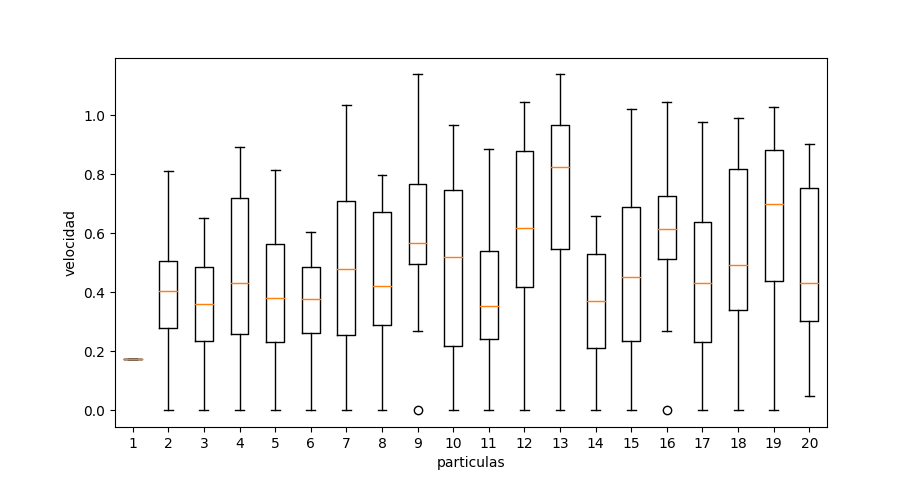
\includegraphics[scale=.7]{caja_bigote.png}
  \caption{Gráfica caja-bigote de velocidades de cada partícula.}
  \label{f1}
\end{figure}
\bigskip

La figura \ref{f2} y figura \ref{f3} muestran gráficamente en puntos la masa por partícula y la carga, la carga por partícula se distribuye en rangos de menos uno a uno para tener distintos niveles de atracción y repulsión.
\begin{figure}[H]
  \centering      
  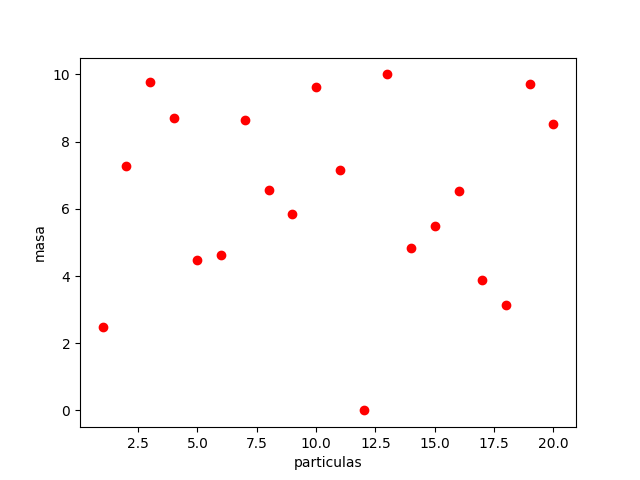
\includegraphics[scale=.7]{particulas_carga.png}
  \caption{Gráfica de masa por cada partícula.}
  \label{f2}
\end{figure}
\bigskip

\begin{figure}[H]
  \centering      
  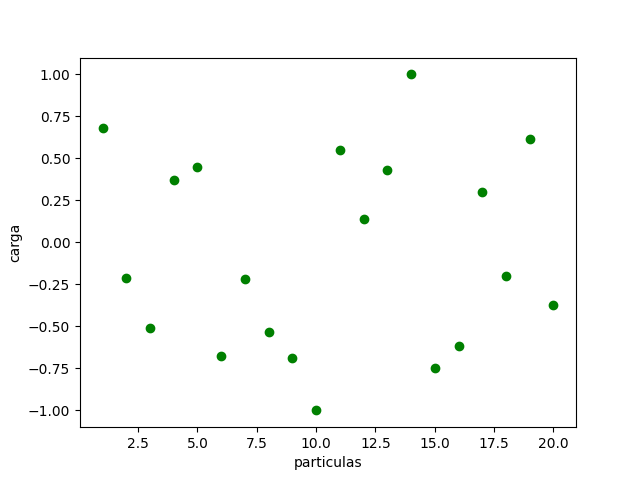
\includegraphics[scale=.7]{particulas_masa.png}
  \caption{Gráfica de carga por cada partícula.}
  \label{f3}
\end{figure}
\bigskip

\section{Conclusión}
La adición de la masa en cada partícula es significativo para la velocidad ya que aumenta el nivel de atracción pero tiene mucha importancia la posición en la que se sitúan ya que en posición más alejada, la atracción no sera la misma que las partículas que estén mas juntas.

\bibliography{refere}
\bibliographystyle{plainnat}

\end{document}
